% Template file for an a0 portrait poster.
% Written by Graeme, 2001-03 based on his SOC poster.
%
% See discussion and documentation at
% <http://www.astro.gla.ac.uk/users/norman/docs/posters/> 
%
%%%%%%%%%%%%%%%%%%%%%%%%%%%%%%%%%%%%%%%%
% Modified by Jozef Dobo\v{s} (c) 2011 % 
%%%%%%%%%%%%%%%%%%%%%%%%%%%%%%%%%%%%%%%%

\documentclass[a0,portrait]{a0poster}
% You might find the 'draft' option to a0 poster useful if you have
% lots of graphics, because they can take some time to process and
% display. (\documentclass[a0,draft]{a0poster})

\pagestyle{empty}
\setcounter{secnumdepth}{0}
\usepackage[absolute,
					%showboxes
					]{textpos}
\usepackage{txfonts}
\usepackage{wrapfig,times}
\usepackage[scaled]{helvet}
\usepackage{graphicx}
\usepackage{forloop}
\usepackage[margin=0cm]{geometry}
\usepackage{wasysym}
\usepackage{enumitem}
\usepackage{tipa}
\usepackage{tikz}
\usetikzlibrary{backgrounds}
\usepackage{cleveref}


%%%%%%%%%%
% Colors %
%%%%%%%%%%
\usepackage{color}
\definecolor{TitleColor}{rgb}{1,1,1} % white
\definecolor{BannerOneColor}{rgb}{0,0,0} % pitch black
\definecolor{BannerTwoColor}{rgb}{0.93,0.08,0.31} % pinky red
\definecolor{BannerThreeColor}{rgb}{0,0.27,0.48} % dark blue
\definecolor{BannerFourColor}{rgb}{0.33,0.19,0.098} % brown
\definecolor{BannerSixColor}{rgb}{0,0.27,0.42} % dark blue
\definecolor{BannerSevenColor}{rgb}{0.62,0.77,0.86} % sky blue
\definecolor{BannerEightColor}{rgb}{0.35,0.33,0.01} % military green
\definecolor{BannerNineColor}{rgb}{0.85,0.86,0.34} % lime green
\definecolor{BannerTenColor}{rgb}{0,0.66,0.80} % strong blue
\definecolor{BannerElevenColor}{rgb}{0.46,0,0.20} % maroon
\definecolor{BannerTwelveColor}{rgb}{0.37,0.32,0.44} % dark washed violet
\definecolor{BannerThirteenColor}{rgb}{0.79,0.84,0.65} % light washed green
\definecolor{BannerFourteenColor}{rgb}{0.57,0.64,0.27} % dark washed green
\definecolor{BannerFifteenColor}{rgb}{0.92,0.91,0.88} % unusable washed 
\definecolor{BannerSixteenColor}{rgb}{0.94,0.36,0.14} % strong orange
\definecolor{BannerSeventeenColor}{rgb}{0.97,0.61,0.19} % orange
\definecolor{BannerEighteenColor}{rgb}{0.99,0.76,0.11} % mustard yellow
\definecolor{BannerNineteenColor}{rgb}{0.79,0.76,0.73} % light gray-ish
\definecolor{BannerTwentyColor}{rgb}{0.63,0.58,0.54} % dark gray-ish

\def\bannercolor{BannerSixColor}

\newcommand{\TODO}[1]{{\color{red}\textbf{[TODO #1]}}}

%%%%%%%%%%%%%%%%%%%%%%%%%%%%%%%%%%%%%%%%%%%%%%%%%%%%%%
% Only change here to affect all headings            %
\newcommand{\headingcolor}{\color{BannerSixColor}} 
\newcommand{\titlecolor}{\color{TitleColor}}
%\newcommand{\banner}{\includegraphics[width=\linewidth]{banners/darkblue.pdf}}
\newcommand{\banner}{\LARGE \tikz{\path[draw=\bannercolor,fill=\bannercolor] (0,0) rectangle (\linewidth,2.25em);}}
\def\Highlight#1{{\sffamily \headingcolor #1}}
%%%%%%%%%%%%%%%%%%%%%%%%%%%%%%%%%%%%%%%%%%%%%%%%%%%%%%

% see documentation for a0poster class for the size options here
\let\Textsize\Large
\def\Head#1{\noindent\hbox to \hsize{\hfil{\LARGE \headingcolor #1}}\bigskip}
\def\LHead#1{\noindent{\sffamily \LARGE \headingcolor #1}\smallskip}
\def\Authors#1{\noindent{\sffamily \LARGE #1}\smallskip}
\def\Subhead#1{\noindent{\large \headingcolor #1}}
\def\Title#1{\noindent{\sffamily \VeryHuge \titlecolor #1}}

\setlist[itemize,1]{topsep=0pt, itemindent=1cm, labelsep=1cm, label={{\headingcolor $\bullet$}}}
\setlist[itemize,2]{topsep=0pt, itemindent=2cm, labelsep=1cm, label={{\headingcolor $\triangleright$}}}
\setlist[itemize,3]{topsep=0pt, itemindent=3cm, labelsep=1cm, label={{\headingcolor -}}}
%\setitemize{topsep=0pt}

% Set up the grid
%
% Note that [0cm,0cm] is the margin round the edge of the page --
% it is _not_ the grid size. That is always defined as 
% PAGE_WIDTH/HGRID and PAGE_HEIGHT/VGRID. In this case we use
% 25 x 25. This gives us three wide columns for text (7 grid
% spacings) and four narrow columns (1 each) at each side of these 
% text columns
%
% Note however that texblocks can be positioned fractionally as well,
% so really any convenient grid size can be used.
%

% [margin, margin]{rows}{cols}
\TPGrid[0cm,0cm]{17}{25}  % 1 - 7 - 1 - 7 - 1 Columns


% Mess with these as you like
\parindent=0pt
%\parindent=1cm
\parskip=0.5\baselineskip
\linespread{1.2}

% abbreviations
\newcommand{\ddd}{\,\mathrm{d}}

\begin{document}

% Understanding textblocks is the key to being able to do a poster in
% LaTeX. In
%
%    \begin{textblock}{width}(x,y)
%    ...
%    \end{textblock}
%
% the first argument gives the block width in units of the grid
% cells specified above in \TPGrid; the second gives the (x,y)
% position on the grid, with the y axis pointing down.

%%%%%%%%%%%%%%
% Top Banner %
%%%%%%%%%%%%%%


%\begin{tikzpicture}[remember picture, overlay]
%\begin{pgfonlayer}{background}
%  \path[draw=BannerTwelveColor,fill=BannerTwelveColor] (0,0) rectangle (\paperwidth,9cm);
%\end{pgfonlayer}
%\end{tikzpicture}

 %if you change this part, you can get matching color for headings
 %in Colors section above
\begin{textblock}{17}(0,0) {
%\includegraphics[width=\paperwidth]{banners/darkblue.pdf}
%\includegraphics[width=\paperwidth]{banners/purple.pdf}
\VeryHuge
\tikz{\path[draw=\bannercolor,fill=\bannercolor] (0,0) rectangle (\paperwidth,3.5em);}
} \end{textblock}




%%%%%%%%%
% Title %
%%%%%%%%%
%TODO MAKE TITLE BANNER BIGGER/LESS CRAMPED
\begin{textblock}{10}(1,0.5)
{\color{TitleColor}
\Title{A CAPT tool for training and research on lexical stress errors in German}\\

%\Authors{Anjana Vakil}, {\sffamily \Large Computational Linguistics}\\
%\textbf{\large \texttt{anjanav@coli.uni-saarland.de}}
}
\end{textblock}

\begin{textblock}{4}(12,0.25)    
\begin{flushright}
%\resizebox{1.5\TPHorizModule}{!}{

\includegraphics[width=1.3\TPHorizModule]{../../../img/new-owl-white.png}
%
\includegraphics{images/saarland_university_white.png}
%
\includegraphics{images/uds-logo-text-white.png}
\end{flushright}
\end{textblock}

\begin{textblock}{4}(10.5,0.5){
\color{TitleColor}
\begin{flushright}
\Authors{Anjana Vakil}\\
{\sffamily \Large Computational Linguistics}\\%, Saarland University}\\
{\sffamily \Large Saarland University}\\
\textbf{\large \texttt{anjanav@coli.uni-saarland.de}}
\end{flushright}
}
\end{textblock}

%\begin{textblock}{5}(1,2){
%\headingcolor
%\Authors{Anjana Vakil}\\
%{\sffamily \Large Computational Linguistics, Saarland University}\\%, U. Saarland}\\
%\textbf{\large \texttt{anjanav@coli.uni-saarland.de}}
%}
%\end{textblock}


%\section{Introduction}

% An example text block, to get you started!
\begin{textblock}{7}(1, 2.75) {
\banner
} \end{textblock}
\begin{textblock}{6.75}(1.25,3){
  \LHead{\titlecolor Overview}}
 \end{textblock}
 \begin{textblock}{7}(1, 3.75)
  \Textsize
%This poster presents the prototype Computer-Assisted Pronunciation Training (CAPT) tool \Highlight{de-stress}: the German (\Highlight{de}) \Highlight{S}ystem for \Highlight{T}raining and \Highlight{R}esearch on \Highlight{E}rrors in \Highlight{S}econd-language \Highlight{S}tress [1].
%
%\Highlight{de-stress} targets lexical stress errors by non-native (L2) German speakers with French as their native language (L1). 
%Its modular design incorporates various methods for diagnosing and presenting feedback on these errors, as described below. 
%
%Both instructional and research applications have motivated the development of \Highlight{de-stress}:

\Highlight{de-stress}: the German (\Highlight{de}) \Highlight{S}ystem for \Highlight{T}raining and \Highlight{R}esearch on \Highlight{E}rrors in \Highlight{S}econd-language \Highlight{S}tress [1] 
is a prototype Computer-Assisted Pronunciation Training (CAPT) tool
aimed at native French speakers learning German as a foreign language. 
The tool targets lexical stress errors (e.g. stressing the wrong syllable in a given word).

The modular design of \Highlight{de-stress} incorporates various methods for diagnosing and presenting feedback on these errors, as described below. Both instructional and research applications have motivated the tool's development:

\begin{itemize}
\item{Learners can receive feedback without human instructor}
\item{Teachers can create exercises matching individual student needs}
%\item{Teachers can create bespoke exercises for students}
\item{Researchers can study efficacy of various diagnosis/feedback types}
%\item{Tool could become useful component of intelligent CAPT system (see \cref{fig:hourglass-ITS})}
\end{itemize}

%  \begin{itemize}
%  \item{helps learners improve their pronunciation without assistance from a human instructor}
%  \item{enables teachers to create exercises matching the individual needs of their students (e.g. proficiency, learning style)}
%    \item{facilitates research into the effectiveness of different diagnosis/feedback methods}
%  \end{itemize}
  

Once more is known about which diagnosis/feedback types are most effective in which situations, this tool could become a useful component of an intelligent CAPT system (see \cref{fig:hourglass-ITS}).


%\Highlight{Context:} M.Sc. thesis, related to ongoing Franco-German project\\ \textit{Individualized Feedback for Computer-Assisted Spoken Language\\ Learning} (IFCASL) [3].
%% at University of Saarland (Saarbr{\"u}cken, Germany) and LORIA (Nancy, France).

\vspace{1em}

	\begin{figure}
	\centering
	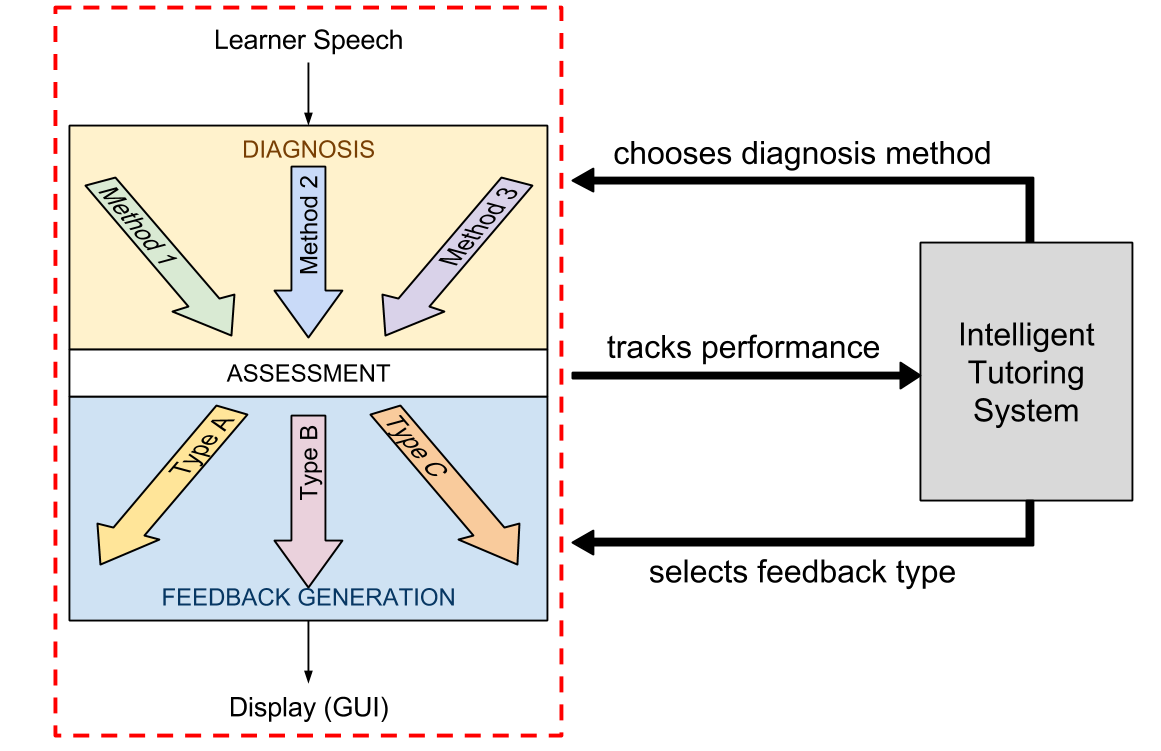
\includegraphics[width=\textwidth]{hourglass-slate}
	\caption{Conceptual diagram of \Highlight{de-stress} (within dashed line) and its possible function in the context of an Intelligent Tutoring System (ITS).}
	\label{fig:hourglass-ITS}
	\end{figure}
 
\end{textblock}


%\section{Training tool}

\begin{textblock}{7}(1, 16.25) {
\banner
} \end{textblock}
\begin{textblock}{6.75}(1.25,16.5){
  %\LHead{\titlecolor A training tool for German learners}}
  \LHead{\titlecolor Error diagnosis}}
 \end{textblock}
 \begin{textblock}{7}(1, 17.25)
\Textsize

A simple web interface presents a learner with a German sentence to read aloud, with one word highlighted as the target for that exercise. The learner submits an utterance of the sentence for assessment. The learner's  realization of the target word's lexical stress pattern is diagnosed via one of the following options:


%\Highlight{Diagnosis options:}
\begin{itemize}[itemsep=.8em]
\item{\Highlight{Classification} using machine learning [2]. Possible feature sets:
	\begin{itemize}
%	\item{Prosodic features of syllables/vowels:
%		\begin{itemize}
%		\item{Duration}
%		\item{Fundamental frequency (F0)}
%		\item{Intensity}
%		\end{itemize}
%	}
	\item{Syllable-level prosodic features  (extracted with JSnoori [3]):
		\begin{itemize}
		\item{Duration}
		\item{Fundamental frequency (F0)}
		\item{Intensity}
		\end{itemize}
	}
	\item{Word uttered}
	\item{Speaker age/gender/proficiency}
	\end{itemize}
}
\item{\Highlight{Comparison} to reference (native-speaker) utterance(s). Options:
	\begin{itemize}
	\item{One-to-one learner-to-reference comparison using JSnoori [3]}
	\item{One-to-many comparison (averaging one-to-one results)}
	\item{Manual reference selection by either instructor or student}
	\item{Automatic reference selection based on F0 mean and range}
	\end{itemize}
}
\end{itemize}





\begin{textblock}{7}(9, 2.75) {
\banner
} \end{textblock}
\begin{textblock}{6.75}(9.25,3){
  \LHead{\titlecolor Feedback delivery}}
 \end{textblock}
 \begin{textblock}{7}(9, 3.75)
  \Textsize
  
  Based on the error diagnosis, one or more of the following types of feedback are presented to the learner via the web interface. %(see \cref{fig:feedback}). 

\vspace{1em}

	\begin{figure}
	\centering
	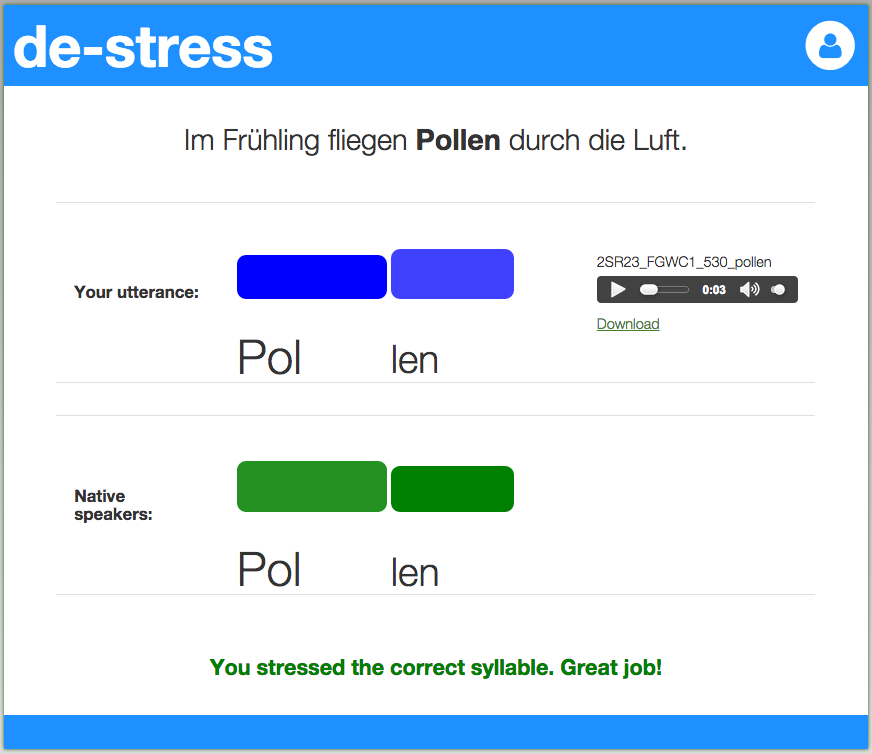
\includegraphics[width=.75\textwidth]{../../../img/screenshots/StudentInterface-userIcon}
	\caption{Feedback via graphical visualization (blue/green rectangles), text stylization (syllable text below rectangles), 
	%learner utterance playback (audio controls), 
	and verbal message (green text).}
	\label{fig:feedback}
	\end{figure}
  

  
  \begin{itemize}
	  \item{\Highlight{Explicit feedback}:
	  	\begin{itemize}
	  		\item{Verbal error/success messages (see \cref{fig:feedback})}
	  		\item{Graphical ``skill bars'' %depicting prosodic parameters (with comparison-based diagnosis only)
	  		}
	  	\end{itemize}
	  }
  \end{itemize}
  
  \begin{figure}
  	\centering
	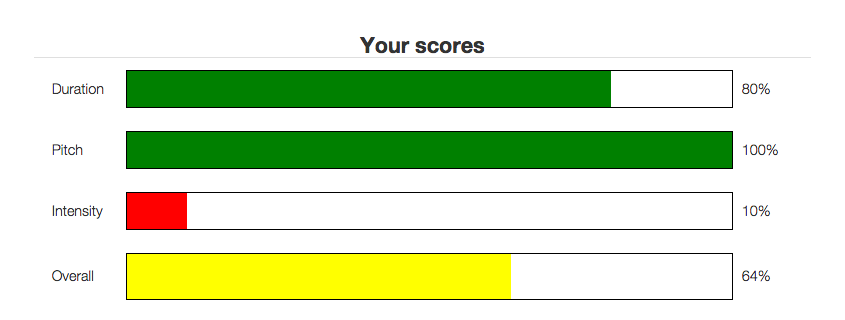
\includegraphics[width=.7\textwidth]{../../../img/screenshots/skillBars-balanced-pct}
	\caption{Feedback via skill bars.}
  \end{figure}
  
  \begin{itemize}
  \item{\Highlight{Implicit feedback} (see \cref{fig:feedback}):
%  	\begin{itemize}
%  	\item{\Highlight{Visual} (see \cref{fig:feedback}):
  %\item{\Highlight{Implicit visual feedback} (see \cref{fig:feedback}): 
	  	\begin{itemize}
	  	\item{Graphical visualization of syllable prosody}
	  	\item{Text stylization reflecting syllable duration}
	  	\end{itemize}
	}
	%\item{\Highlight{Auditory}: 
%  \item{\Highlight{Implicit auditory feedback}:
%		\begin{itemize}
%		\item{Original learner and reference utterances (see \cref{fig:feedback})}
%		\item{Prosodically modified learner utterance (using JSnoori [3])}
%		\end{itemize}
%  	}
  	%\end{itemize}
  %}
  \item{\Highlight{Self-assessment} questionnaire for learner to complete % before receiving other feedback
  }
  \end{itemize}




\end{textblock}
  
  \end{textblock}
  
  
  
  %\section{Teaching and research tool}

  
  \begin{textblock}{7}(9, 16.25) {
\banner
} \end{textblock}
\begin{textblock}{6.75}(9.25,16.5){
  \LHead{\titlecolor Administrative interface for teachers/researchers}}
 \end{textblock}
 %\begin{textblock}{7}(9, 18)
 \begin{textblock}{3.85}(12,17.2)
  
  	\begin{figure}
	%\centering
	%\fcolorbox{gray!50}{white}{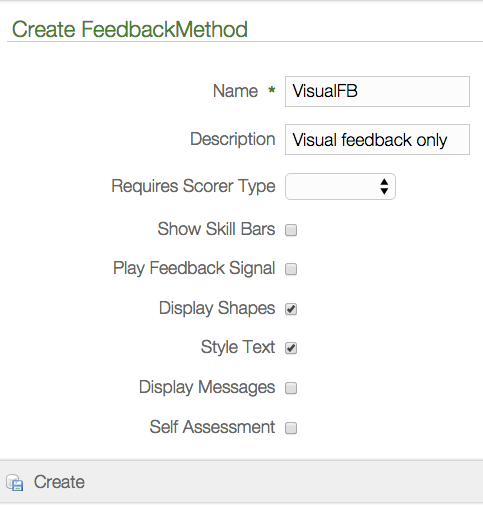
\includegraphics[width=.7\textwidth]{../FeedbackMethod}}
	\fcolorbox{gray!50}{white}{
	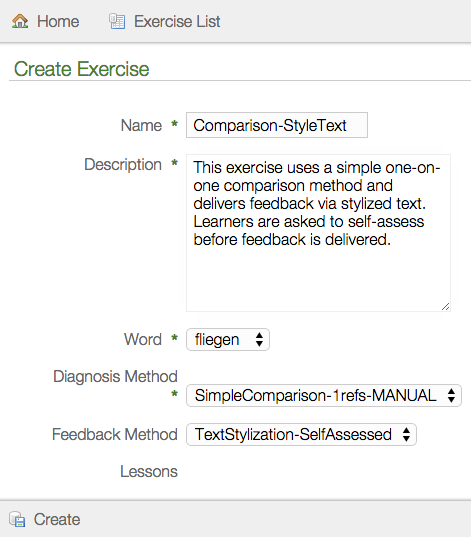
\includegraphics[width=\textwidth]{../../../img/screenshots/TeacherInterface-smaller-er}
	}
	\caption{Admin. interface for creating a new exercise combining specific diagnosis and feedback options.}
	\end{figure}	  
  
 \end{textblock}  
 \begin{textblock}{2.35}(9,17.25)
   \Textsize
  %An administrative interface allows language teachers or CAPT researchers to combine the available diagnostic and feedback method(s) to create new exercises for learners. 
  An administrative interface allows a language teacher or CAPT researcher to  create new exercises for students to complete. Each exercise features a specific combination of the various diagnosis and feedback options described above. %in the system. 
  
%  By allowing straightforward (graphical) yet fine-grained control over these features, \Highlight{de-stress}: 
%  \begin{itemize}
%  \item{enables researchers to create different CAPT exercises for comparative in vivo studies}
%  \item{allows teachers to create exercises matching the individual needs of their students (e.g. proficiency, learning style)}
%  \end{itemize}
  
%  \begin{itemize}
%  \item{Teachers can create exercises targeted to students' needs (learning style, etc.)}
%  \item{Researchers can study impact of various diagnosis/feedback configurations on factors impacting CAPT system success, e.g.
%  \begin{itemize}
%  \item{learning outcomes}
%  \item{user engagement/satisfaction}
%  \end{itemize}
%  }
%  \end{itemize}
 
 
% \vspace{1em}
% 

%  
  
\end{textblock}


%\begin{textblock}{7}(9, 8.5) {
%\banner
%} \end{textblock}
%\begin{textblock}{6.75}(9.25,8.75){
%  \LHead{\titlecolor A teaching and research tool}}
% \end{textblock}
% \begin{textblock}{7}(9, 9.5)
%  \Textsize
% 
%\end{textblock}



%\section{Conclusion}

%% Another text block in the bottom right.
%\begin{textblock}{7}(9,18){
%\banner
%} \end{textblock}
%\begin{textblock}{6.75}(9.25,18.25){
%  \LHead{\titlecolor Conclusion and future directions}
%   } \end{textblock}
% \begin{textblock}{7}(9, 19)
%  \Textsize
%  
%%  Both instructional and research applications have thus motivated the development of \Highlight{de-stress}.
%%Unlike with some existing tools for diagnosis and feedback on pronunciation errors, learners can interact with the tool and interpret its feedback independently, i.e. without the assistance of a human instructor at their side.
%%At the same time, researchers can use this modular system to study the impact of various assessment and feedback types on learner outcomes, user engagement, and other factors impacting the success of a CAPT system. 
%%%
%%Once more is known about which diagnosis/feedback types should be delivered to which learners in which situations, this tool could become a useful component of a fully-fledged intelligent CAPT system, in which 
%%%learner models and other intelligent components
%%models of relevant aspects of the learning context (e.g. the student's skill level, progress, or personal preferences; the current learning objective or position in a sequence of exercises; etc.)
%%are used to automatically decide which modules of the tool to activate, as \cref{fig:hourglass-ITS} illustrates.
%  
%  
%  
%\end{textblock}



%\section{References}

%\begin{textblock}{7}(9,22.5){
%\banner
%} \end{textblock}
%\begin{textblock}{6.75}(9.25,22.75){
%  \LHead{\titlecolor References}
%   } \end{textblock}
% \begin{textblock}{7}(9, 23.3)

\begin{textblock}{7}(9,22.75)
{\Large
\tikz{\path[draw=\bannercolor,fill=\bannercolor] (0,0) rectangle (\linewidth,2em);}}
\end{textblock}
\begin{textblock}{6.75}(9.15,22.95){
  \LHead{\Large \titlecolor References}
   } \end{textblock}
 \begin{textblock}{7}(9, 23.3)
%  \Textsize
%  
%  
%\end{textblock}
%
%
%\begin{textblock}{15}(1,23)
%{\Large
%\tikz{\path[draw=\bannercolor,fill=\bannercolor] (0,0) rectangle (\linewidth,2em);}}
%\end{textblock}
%\begin{textblock}{14.75}(1.15,23.15)
%\LHead{\Large \titlecolor References}
%\end{textblock}
%\begin{textblock}{15}(1,23.55)

\begin{enumerate}[label={[\arabic*]}, leftmargin=34pt, topsep=0pt]

\item{
	%A. S. Vakil, "de-stress," 
	\texttt{http://github.com/vakila/de-stress}%
	%.
	}

\item{A. S. Vakil and J. Trouvain, "Automatic classification of lexical stress errors for German CAPT," in \textit{SLaTE}, 2015.}

\item{
	%LORIA Speech Team, "JSnoori," 
	\texttt{http://jsnoori.loria.fr}%
	%.
	}



%\item{Trouvain, J., et al. 2013. ``Designing a bilingual speech corpus for French and German language learners''. \textit{Proc. Corpus et Outils en Linguistique, Langues et Parole}, Strasbourg, pp. 32-34.}
\end{enumerate}

\end{textblock}

%\begin{textblock}{15}(1,23.25)
%\LHead{\Large \headingcolor References}
%\begin{enumerate}[label={[\arabic*]}, leftmargin=34pt, topsep=0pt]
%\item{Bonneau, A. and V. Colotte. 2011. “Automatic Feedback for L2 Prosody Learning”. In \textit{Speech and Language Technologies}. Ivo Ipsic, ed. InTech.}
%
%\item{Hirschfeld, U. 1994. \textit{Untersuchungen zur phonetischen Verst{\"a}ndlichkeit Deutschlernender.} Forum Phoneticum, 57.}
%
%\item{Trouvain, J., et al. 2013. ``Designing a bilingual speech corpus for French and German language learners''. \textit{Proc. Corpus et Outils en Linguistique, Langues et Parole}, Strasbourg, pp. 32-34.}
%\end{enumerate}
%
%\end{textblock}


% If you want to add a figure do something like this:

%\begin{textblock}{3}(1,15)
%  \begin{center}
%  \resizebox{3\TPHorizModule}{!}{\includegraphics{images/group-logo.pdf}}
%\\{\bfseries Figure 5:} caption
%  \end{center}
%\end{textblock}



% Place the group logo at the bottom left - visually this balances
% well with the University logo at the top right. 
%\begin{textblock}{4}(1,23)    
%%\resizebox{1.5\TPHorizModule}{!}{
%
\includegraphics{images/uds-logo-text.png}
%%}
%\end{textblock}



\end{document}

